% \UPSTIobjectif{

% }
\section{Rappels sur la programmation orientée objet}
\subsection{Quelques définitions}

La programmation orientée objet est une technique de programmation qui consiste à découper un programme en plusieurs objets qui interagissent entre eux. 
Chaque objet est une instance d'une classe. Une classe est un ensemble d'attributs et de méthodes. Les attributs sont des variables propres à chaque objet. Les méthodes sont des fonctions propres à chaque objet.

%%%% Idée %%%%
Il s'agit d'une façon de penser la programmation. Si elle peut paraître plus complexe au début, elle permet de structurer le code, de le rendre plus lisible et plus facilement modifiable. 

La définition des objets (création de classes) peut être complexe, mais l'utilisation des objets est largement simplifiée. C'est d'ailleurs un avantage majeur de la programmation orientée objet : l'utilisateur d'un objet n'a pas besoin de connaître sa définition pour l'utiliser. Il lui suffit de connaître les méthodes et les attributs de l'objet.

%%%% /Idée %%%%

%%%% Explication %%%%
Un object est une instance d'une classe. Cela veut simplement dire qu'une classe définit une structure (attributs et méthodes) et qu'un objet est un cas particulier de cette structure. Par analogie, on peut parler des plans d'une maison qui définissent ce qu'est une maison (nombre de pièces, surface, etc.) et des maisons qui sont des instances de ces plans. 

Chaque maison pourra avoir un nombre de pièces différentes, une couleur de toit différente, mais toutes les maisons auront les mêmes caractéristiques de base (elles auront toutes un toit, des pièces, des murs, des fenêtres, etc.).

\begin{center}
    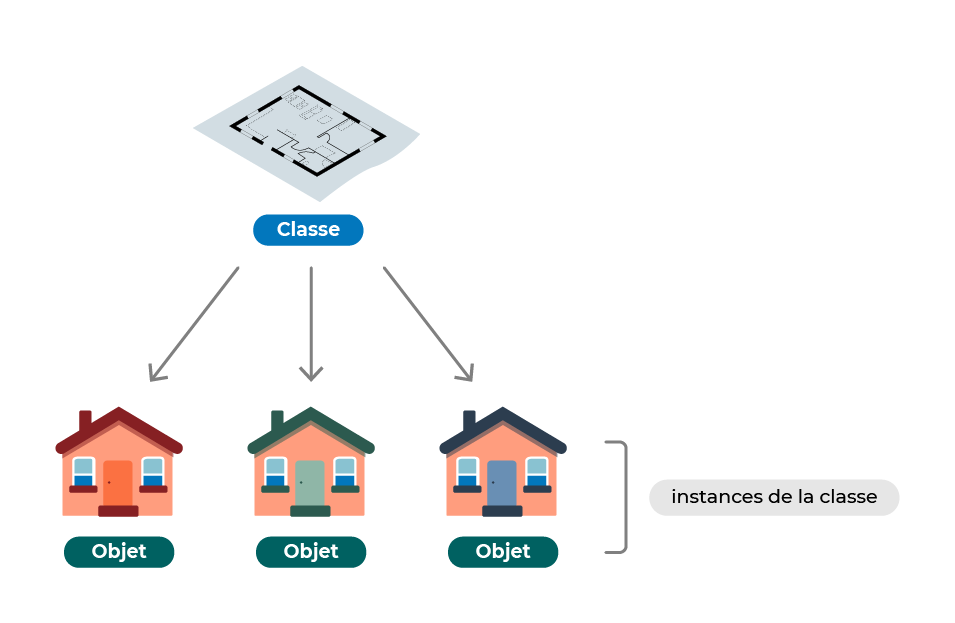
\includegraphics[width=.8\textwidth]{classe_exemplePlanMaison.png} 
\end{center}

%%%% /Explication %%%%
